\documentclass{mini}
\usepackage[utf8]{inputenc}
\usepackage{fancyvrb}
\usepackage{amsmath}
\newcommand{\degree}{\ensuremath{^\circ}}
\newcommand{\hilight}[1]{\colorbox{yellow}{#1}}
\linespread{1.5}
\DeclareUnicodeCharacter{00A0}{~}

%------------------------------------------------------------------------------%
\title{Analiza możliwości wykorzystania w~algorytmie CMA-ES wiedzy o~ograniczeniach kostkowych}

\author{inż. Robert Jakubowski}
\supervisor{dr hab. inż. Jarosław Arabas prof. nzw. PW}
\type{magisters}
\monthyear{Maj 2016}
\date{\today}
\album{237545}
%------------------------------------------------------------------------------%
\begin{document}

\maketitle

\pagebreak
\thispagestyle{empty}

\openup -0.2em %make it fit on one page
\tableofcontents 
\openup 0.2em %make it fit on one page

\thispagestyle{empty}
\raggedbottom
\pagebreak


\section{Streszczenie}

\pagebreak

\section{Wstęp}

\subsection{Cel pracy}

\pagebreak

\section{Techniki uwzględniania ograniczeń}
Niektóre problemy optymalizacyjne posiadają ograniczenia. Szukając rozwiązania należy zapewnić, że rozwiązanie będzie dopuszczalne. Zgodnie z --------łącze-------- techniki, które w tym pomagają można podzielić w następujący sposób:
\begin{itemize}[noitemsep]
\item definicja przestrzeni przeszukiwań - zapewnienie, że podczas krzyżowań, mutacji i innych zmian punktów, żaden z punktów nie wypadnie poza przestrzeń przeszukiwań,
\item modyfikacja funkcji celu - zmienienie funkcji celu tak, aby funkcja celu dla punktów spoza ograniczeń zwracały gorsze wyniki,
\item transformacja rozwiązań - punkty, które są poza ograniczeniami zostają zamieniane na punkty, które znajdują się w ograniczeniach.
\end{itemize}

W tej pracy skupiono się na transformacji rozwiązań

\subsection{Transformacje rozwiązań} \label{transformacje}
Nie istnieje jedna technika transformacji rozwiązań spoza ograniczeń, na dopuszczalne. W kolejnych podrozdziałach opisane są metody transformacji rozwiązań, które były badane. Każda z technik jest opisana słownie oraz pseudokodem. Opis słowny zawiera wyjaśnienie, co się dzieje z punktem, który znalazł się poza ograniczeniem. W pseudokodzie zastosowane następujące oznaczenia:
\begin{itemize}[noitemsep]
\item $x$ - punkt, który poddajemy naprawie
\item $x'$ - ojciec punktu $x$, czyli z punktu $x'$ z zadanym rozkładem został wylosowany punkt $x$
\item $x(i)$ - wartość $i$-tej współrzędnej punktu $x$
\item $lb$ - ograniczenie dolne
\item $ub$ - ograniczenie górne
\end{itemize}

\subsubsection{Powrót?}
Nowy punkt zostaje odrzucony i wraca do poprzedniej pozycji.

\begin{Verbatim}[baselinestretch=1.1]
	x = x'
\end{Verbatim}


\subsubsection{Rzutowanie}
Punkt jest transformowany do najbliższego punktu, który spełnia ograniczenie. Oznacza to, że dla każdej współrzędnej sprawdzany jest warunek zawierania się w ograniczeniach. Dla współrzędnych, dla których nie jest on spełniony, wartość jest zamieniana na wartość ograniczenia (dolnego lub górnego), które jest najbliżej.

\begin{Verbatim}[baselinestretch=1.1]
	dla każdej współrzędnej i
		jeżeli lb(i) > x(i)
			x(i) = lb(i)
		jeżeli ub(i) < x(i)
			x(i) = ub(i)
\end{Verbatim}

\subsubsection{Reinicjalizacja}
Punkt jest przenoszony do pozycji początkowej. W tej pracy był to jednocześnie środek układu współrzędnych oraz środek symetrii ograniczeń.

\begin{Verbatim}[baselinestretch=1.1]
	x = x0
\end{Verbatim}


\subsubsection{Odbicie}
Dla każdej współrzędnej sprawdzane są warunki na ograniczenie. W przapadku współrzędnych, na których punkt jest poza ograniczeniem, wartość punktu tej współrzędnej jest symetrycznie odbita względem ograniczenia, którego warunek został złamany.

\begin{Verbatim}[baselinestretch=1.1]
	dla każdej współrzędnej i
		jeżeli lb(i) > x(i)
			x(i) = x(i) + 2 * (lb(i) - x(i))
		jeżeli ub(i) < x(i)
			x(i) = x(i) - 2 * (x(i) - ub(i))
\end{Verbatim}

\subsubsection{Próbkowanie}
Punkt jest powtórnie losowany dopóty, dopóki spełnia ograniczenia kostkowe.

\begin{Verbatim}[baselinestretch=1.1]
	dopóki !w_ograniczeniach(x)
		x = losuj(x')
\end{Verbatim}

\subsubsection{Zawijanie}
Dla każdej współrzędnej sprawdzane są warunki na ograniczenie. W przapadku współrzędnych, na których punkt jest poza ograniczeniem, różnica, pomiędzy ograniczeniem a wartością współrzędnej punktu, jest zapamiętywana. Tę różnicę odkładamy na przeciwległym ograniczeniu po stronie, która jest wewnątrz ograniczenia. W tym miejscu znajduje się nowa wartość współrzędnej punktu. W intuicyjny sposób można to wyjaśnijć tak, że dla punktów nie ma ograniczeń, a przestrzeń przeszukiwań po każdym wymiarze jest jakby "zawinięta".

\begin{Verbatim}[baselinestretch=1.1]
	dla każdej współrzędnej i
		jeżeli lb(i) > x(i)
			x(i) = ub(i) - (lb(i) - x(i))
		jeżeli ub(i) < x(i)
			x(i) = lb(i) + (x(i) - ub(i))
\end{Verbatim}

\subsection{Błądzenie przypadkowe} \label{bladzenie}

Można się spodziewać, że algorytm CMA-ES dla funkcji stałej będzie zachowywał się analogicznie do błądzenia przypadkowego. Takie założenie skłoniło autorów, żeby przyjrzeć się błądzeniu przypadkowemu z ograniczeniami. Błądzenie przypadkowe jest algorytmem dużo prostrzym, niż CMA-ES, więc umożliwia szybsze testowanie i wyciąganie wniosków.\\
Niech $ X_1, X_2, ... $ będą niezależnymi n-wymiarowymi zmiennymi losowymi o wartości oczekiwanej równej $ \{0\}^n $. Błądzeniem przypadkowym nazywamy sekwencję zmiennych losowych:
\begin{equation}
S_0 = 0, S_i=X_1+X_2+...+X_i
\end{equation}

\subsection{Metoda przeprowadzania testów}
W celu przeprowadzenia testów napisano szereg skryptów w języku MATLAB. Testy te obserwowały wpływ metod uwzględniania ograniczeń na ruch punktu. W rezultacie miały one pokazać rozkład prawdopodobieństwa punktu dla danej metody. Metody wybrane do testowania są takie jak w podrozdziale \ref{transformacje}.
Ponadto badano 2 różne metody losowania punktów: rozkład normalny oraz jednostajny. W przypadku rozkładu jednostajnego losowano liczby z przedziału $[-0.5; 0.5]$ (przedział zazwyczaj kilkukrotnie krótszy od ograniczeń kostkowych).

\subsubsection*{Skrypty}
Skrypty zostały zbudowane zgodnie z poniższym pseudokodem.
\begin{Verbatim}[baselinestretch=1.1]
	x - błądzący punkt
	punkty - tablica wszystkich położeń punktu x
	iteracje - liczba iteracji podana jako parametr
	i = 0
	dopóki i < iteracje
		wylosuj nowe położenie punktu x
		jeżeli x jest poza ograniczeniem
			popraw x
		dodaj x do tablicy punkty
		i = i + 1
\end{Verbatim}

\subsection{Wyniki testów}

\subsubsection*{Powrót?}
\begin{figure}[H]
\centering
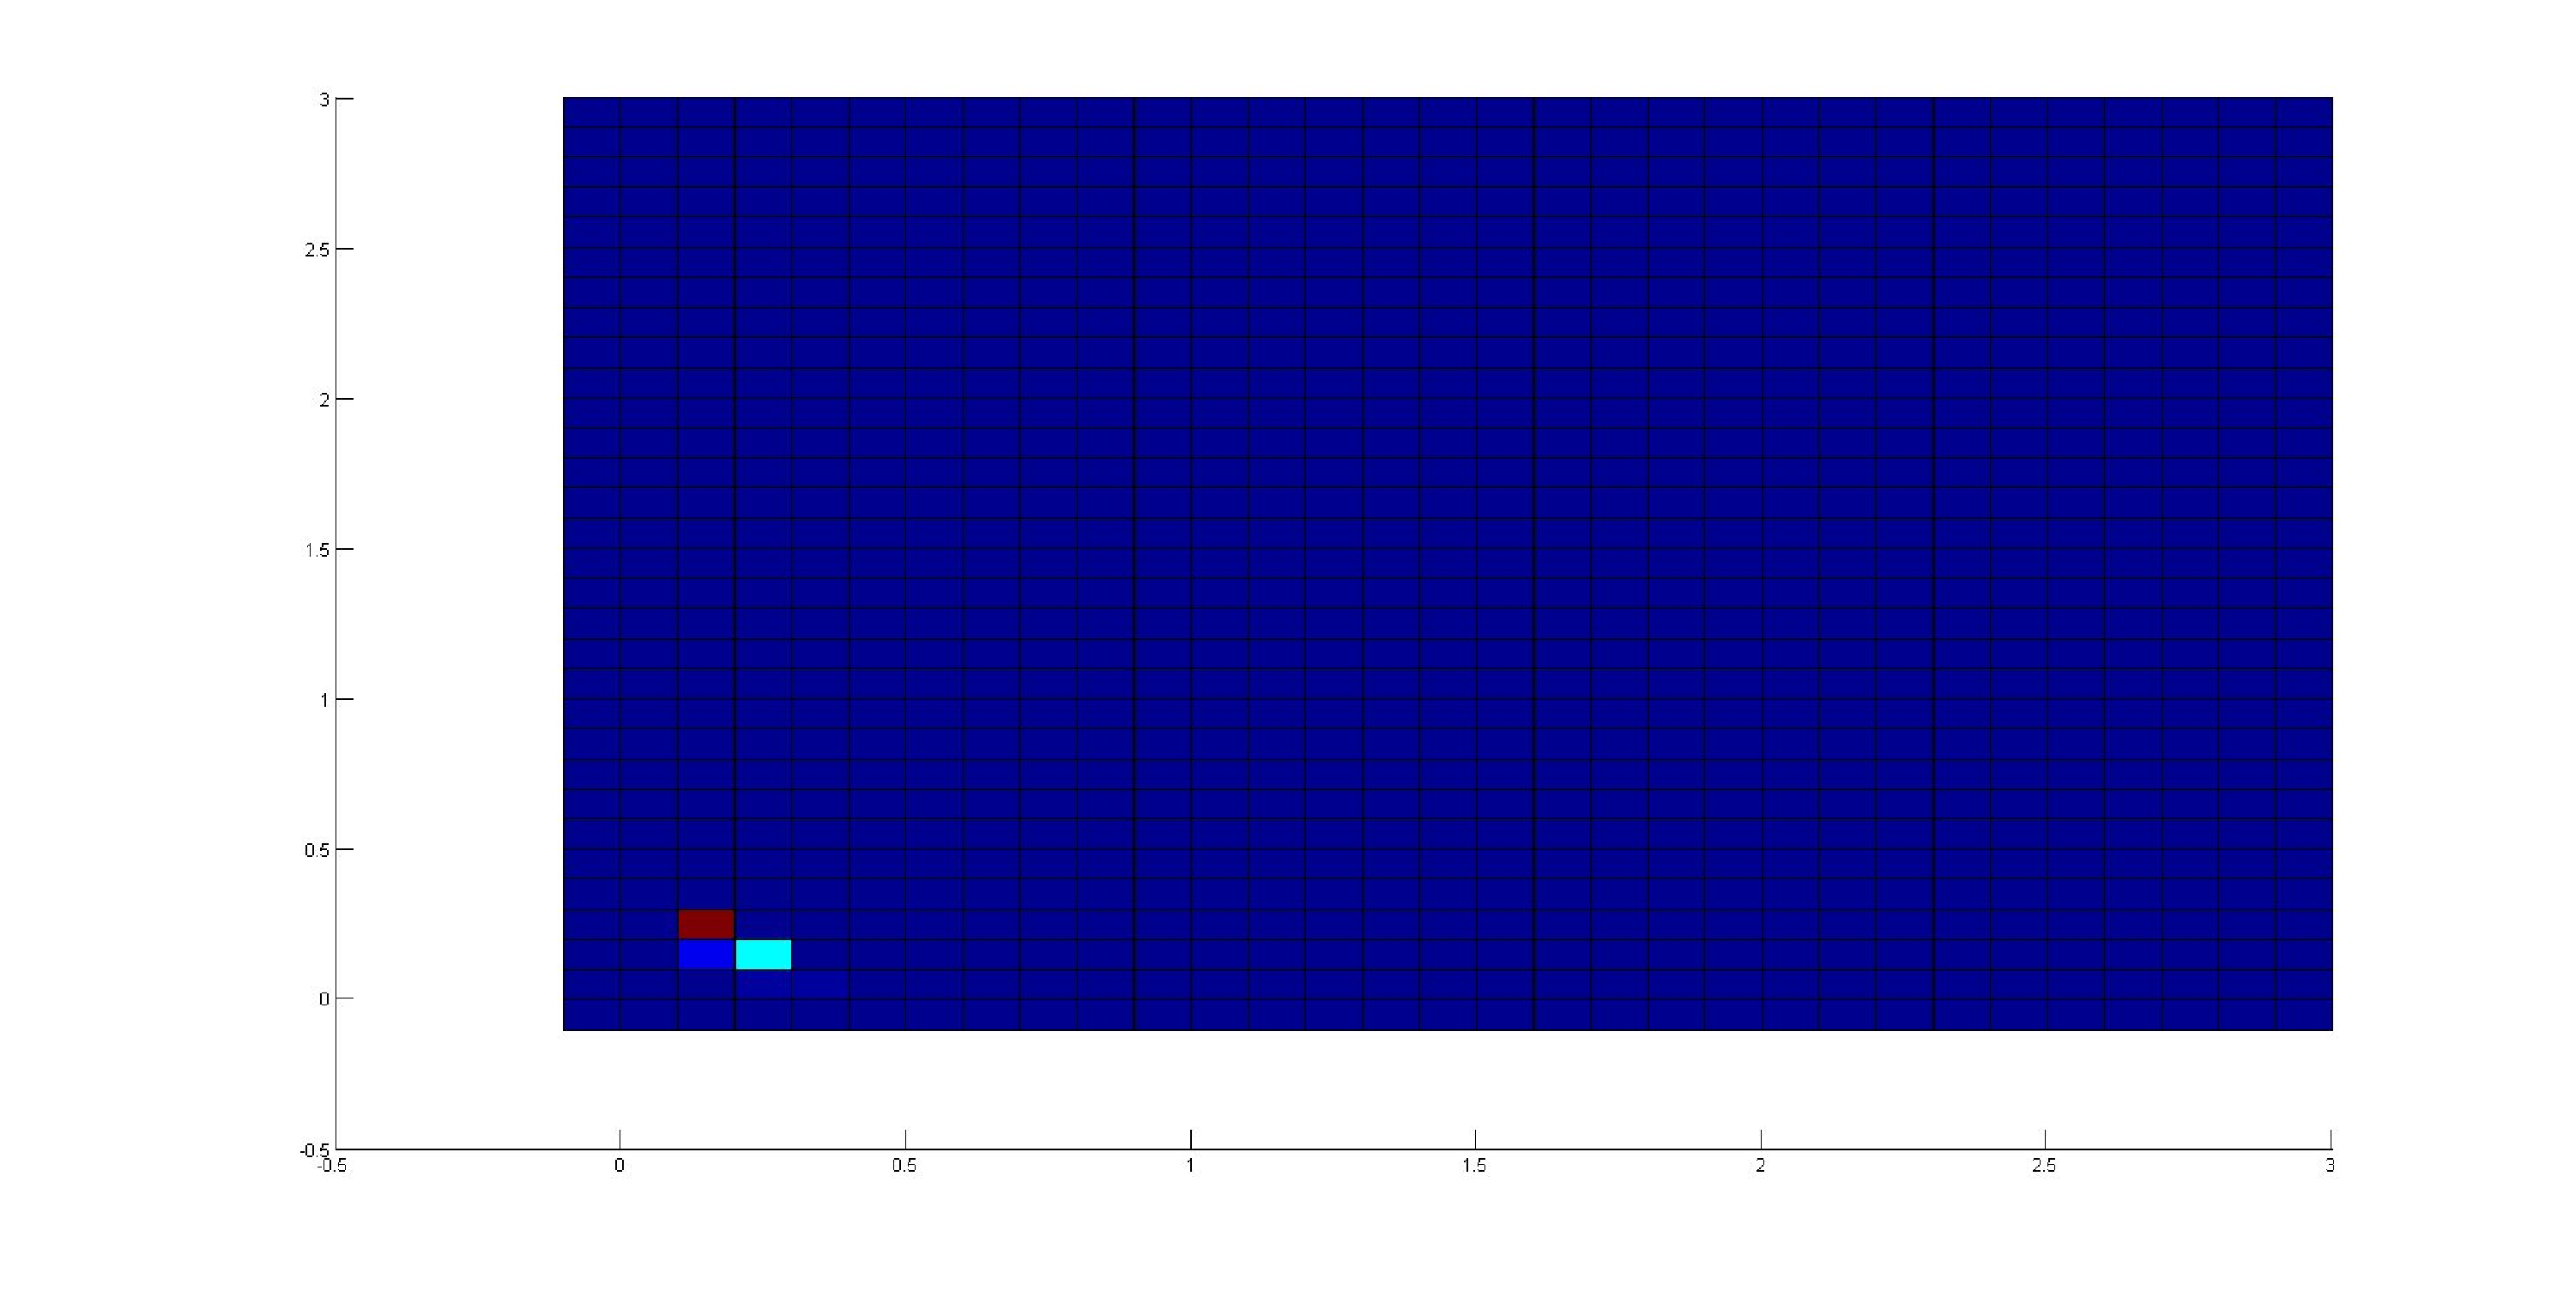
\includegraphics[scale=0.3]{algorytm}
\caption{Dwa kroki algorytmu wykonane dla pojedynczej komórki początkowej}
\label{fig:algorytm}
\end{figure}

\subsubsection*{Rzutowanie}

\subsubsection*{Reinicjalizacja}

\subsubsection*{Odbicie}

\subsubsection*{Próbkowanie}

\subsubsection*{Zawijanie}

\subsection{Wnioski}

\pagebreak

\section{Benchmarki}
Zgodnie z założeniami poczynionymi w rozdziale \ref{bladzenie} testy algorytmu CMA-ES powinny przynieść rezultaty zbliżone do testów błądzenia przypadkowego.

\subsection{Metoda przeprowadzania testów}
Do przeprowadzania testów została użyta biblioteka przygotowana przez Nikolausa Hansena, współautora algorytmu CMA-ES. Podobnie, jak w przypadku błądzenia przypadkowego, wykorzystano implementację w języku MATLAB ---przypis---.

\subsection{Wnioski}

\pagebreak

\section{Wpływ technik na efektywność CMA-ES}

\subsection{Algorytm CMA-ES}
Klasyczne algorytmy ewolucyjne nie dostosowują się do charakterystyki optymalizowanej funkcji. W większości z nich rozkład prawdopodobieństwa losowanych punktów jest stały. Z tego faktu wynika problem dobrania parametrów przeszukiwania. Na przeciw tym problemom wychodzi algorytm CMA-ES, który w swej idei ma dopasowywać się do badanej funkcji.\\
Rozwinięcie akronimu CME-ES podpowiada, w jaki sposób jest to realizowane: Covariance Matrix Adaptation - Evolution Strategy (adaptacja macierzy kowariancji - strategia ewolucyjna). Punkty losowane są na podstawie macierzy kowariancji, która jest w każdej iteracji dostosowywana do aktualnej sytuacji przeszukiwań.

\subsubsection*{Szczegóły}

\pagebreak

\section{Podsumowanie}

\subsection{Wyniki}

\subsection{Możliwości rozwoju}

\pagebreak

\begin{thebibliography}{9}

\end{thebibliography}

\makestatement

\end{document}
